\section{Analysis Settings}
\label{sec:experimental-set-up}
\begin{figure*}[t] %[!b]
    \centering
    \vspace{-10pt}
    %\scalebox{.9}{
    \begin{subfigure}[t]{0.31\linewidth}
        \centering
        \fbox{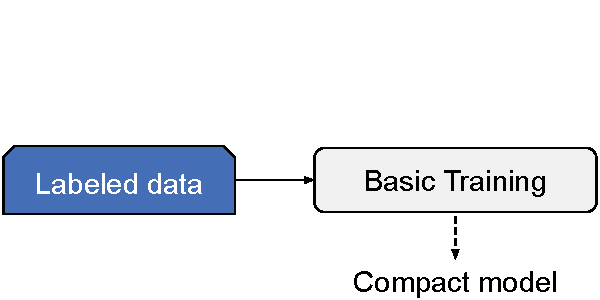
\includegraphics[width=\columnwidth]{figures/recolored_vanilla_training.pdf}}
        \caption{Basic Training}
        \label{fig:baseline-vanilla-training}
    \end{subfigure}
    \hspace{0.3cm}
    \begin{subfigure}[t]{0.31\linewidth}
        \centering
        \fbox{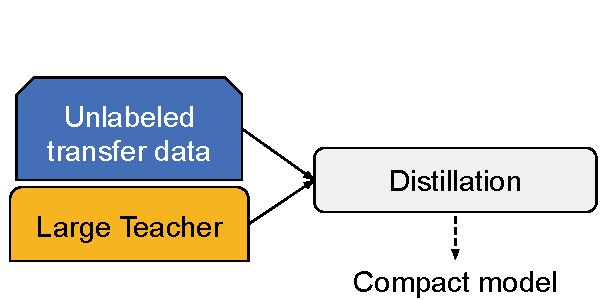
\includegraphics[width=\columnwidth]{figures/recolored_knowledge_distillation.pdf}}
        \caption{Distillation}
        \label{fig:baseline-distillation}
    \end{subfigure}
    \hspace{0.3cm}
    \begin{subfigure}[t]{0.31\linewidth}
        \centering
        \fbox{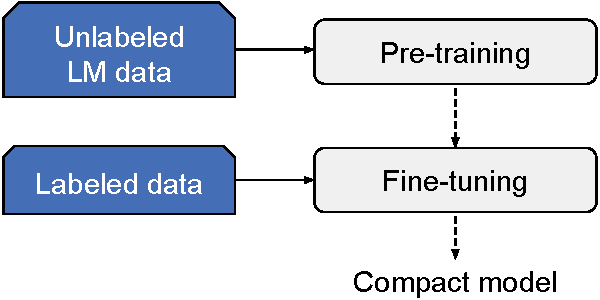
\includegraphics[width=\columnwidth]{figures/recolored_pre-training.pdf}}
        \caption{\PtFt (PF)}
        \label{fig:baseline-pretraining}
    \end{subfigure}
    %}
    \caption{Baselines for building compact models, used for analysis (Section \ref{sec:exp}).}
    \label{fig:training-strategies}
    \vspace{-10pt}
\end{figure*}

Given these positive results, we aim to gain more insight into Pre-trained Distillation. We perform extensive analyses on two orthogonal axes---model sizes and properties of unlabeled data, thus departing from the settings used in Section \ref{sec:concurrent}.

All our models follow the Transformer  architecture~\citep{transformer} and input processing used in BERT~\cite{bert}. We denote the number of hidden layers as $L$ and the hidden embedding size as $H$, and refer to models by their $L/H$ dimensions. We always fix the number of self-attention heads to $H / 64$ and the feed-forward/filter size to $4H$. The end-task models are obtained by stacking a linear classifier on top of the Transformer architectures.

The teacher, \bertlarge, has dimensions 24L/1024H and 340M parameters. We experiment with 24 student models, with sizes and relative latencies listed in Table \ref{tab:bert-models}. The most expensive student, \bertbase, is 3 times smaller and 1.25 times faster than the teacher; the cheapest student, \bertsmall, is 77 times smaller and 65 times faster. For readability, we report results on a selection of 5 students, but verify that all conclusions hold across the entire 24-model grid.

\subsection{Analysis Baselines}

\label{sec:baselines}
We select three baselines for Pre-trained Distillation that can provide insights into the contributions made by each of its constituent operations. 

\textbf{Basic Training} (Figure \ref{fig:baseline-vanilla-training}) is the standard  supervised learning method: a compact model is trained directly on the labeled set.

\textbf{Knowledge Distillation} (Figure \ref{fig:baseline-distillation}) \citep{model-compression,distillation} (or simply ``distillation'') transfers information from a highly-parameterized and accurate \emph{teacher} model to a more compact and thus less expressive \emph{student}. For classification tasks, distillation exposes the student to \emph{soft labels}, namely the class probabilities produced by the teacher 
$p_l = \mbox{softmax}(z_l/T),$
where $p_l$ is the output probability for class $l$, $z_l$ is the logit for class $l$, and $T$ is a constant called \emph{temperature} that controls the smoothness of the output distribution. The softness of the labels enables better generalization than the gold \emph{hard labels}. For each end task, we train: (\textit{i})
    \textbf{a teacher} obtained by fine-tuning pre-trained \bertlarge\ (24L/1024H) on the labeled dataset (note teachers do not learn from the  transfer set), and (\textit{ii}) \textbf{24 students} of various sizes. %
    Students are always distilled on the soft labels produced by the teacher with a temperature of 1\footnote{While \citet{distillation} show that tuning the temperature could increase performance, we did not observe notable gains. They also propose using a weighted sum of the soft and hard labels, but this approach cannot be applied directly in our set-up, since not all instances in our unlabeled transfers set have hard labels. Our optional final fine-tuning step similarly up-weights the hard labels in the labeled set. }.

\textbf{Pre-training$+$Fine-tuning} (Figure \ref{fig:baseline-pretraining}) \citep{first-finetuned-pretraining,bert}, or simply PF, leverages large unlabeled general-domain corpora to pre-train models that can be fine-tuned for end tasks. Following BERT, we perform pre-training with the masked LM (MLM) and next sentence objectives (collectively referred to as MLM$^+$ from here on). The resulting model is fine-tuned on end-task labeled data. While pre-training large models has been shown to provide substantial benefits, we are unaware of any prior work systematically studying its effectiveness on compact architectures.

\subsection{Analysis Tasks and Datasets}
\label{sec:tasks-and-datasets}
\begin{wrapfigure}{r}{0.55\textwidth}
    \vspace{-10pt}
    \small
    \centering
    \begin{tabularx}{0.55\columnwidth}{p{2.7cm}X}
         \toprule
         \textbf{Labeled Data ($\D_L$)} & \textbf{Unlabeled \mbox{Transfer Data ($\D_T$)}} \\
         \midrule
         MNLI (390k) &  \nlistar (1.3m samples)  \\
         RTE (2.5k) & \nlistar (1.3m samples) \\
         SST-2 (68k) & Movie Reviews* (1.7m samples) \\
         Book Reviews (50k) & Book Reviews* (8m samples) \\
         \bottomrule
    \end{tabularx}
    \captionof{table}{\small \textbf{Datasets used for analysis.} A star indicates that hard labels are discarded. NLI* refers to the collection of MNLI (390k), SNLI (570k) and QQP (400k). The reviews datasets are part of Amazon Product Data. Unless otherwise stated, $\D_{LM}$ consists of \BCW. }
    \label{tab:tasks-and-datasets}
    \vspace{-10pt}
\end{wrapfigure}
The tasks and associated datasets are summarized in Table~\ref{tab:tasks-and-datasets}.

\textbf{Sentiment classification} aims to classify text according to the polarities of opinions it contains. We perform 3-way document classification on  Amazon  Book  Reviews~\citep{amazon}.
Its considerable size (8m) allows us to closely follow the standard distillation setting, where there is a large number of unlabeled examples for transfer. Additionally, we test our algorithm on \sst~\citep{sst2}, which is a binary sentence classification task, and our results are directly comparable with prior work on the GLUE leaderboard \citep{glue}. We use whole documents from Amazon Movie Reviews (1.7m) as unlabeled transfer data (note that \sst consists of single sentences).

\textbf{Natural language inference} involves classifying pairs of sentences (a premise and a hypothesis) as \emph{entailment}, \emph{contradiction}, or \emph{neutral}. This task is representative of the scenario in which proxy data is non-trivial to gather \citep{nli_artifacts}. We chose MNLI \citep{mnli} as our target dataset. Since strictly in-domain data is difficult to obtain, we supplement \DT with two other sentence-pair datasets: SNLI \citep{snli} and QQP \citep{qqp}.

\textbf{Textual entailment} is similar to NLI, but restricted to binary classification (\emph{entailment} vs \emph{non-entailment}). The most popular RTE dataset~\citep{rte} is two orders of magnitude smaller than MNLI and offers an extreme test of robustness to the amount of transfer data.